\chapter{Implementation}

In this chapter, the theoretical explanations of the previous chapters are transferred into practical implementations with Python.

\section{Overview}

First, an overview is given to make the implementation easier to follow.

\subsection{Scapy modules for UDS scanning}

\begin{figure}[htb]
    \centering
    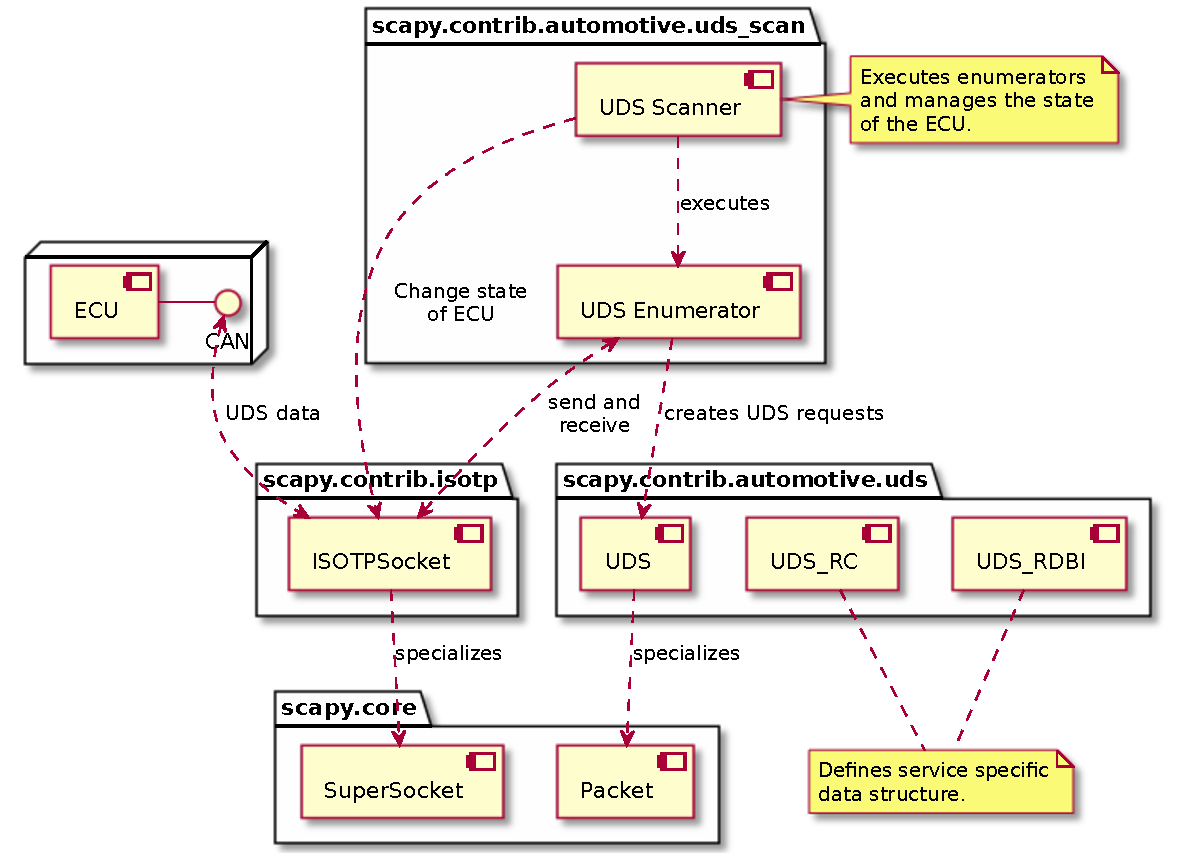
\includegraphics[width=0.83\textwidth]{uml/context}
    \caption{Interconnected modules of Scapy for UDS scanning.}
    \label{fig:uml-context}
\end{figure}

Scapy is a large program with many functions for all possible use cases. For a UDS scan, its modules shown in \autoref{fig:uml-context} are used together. Basically it needs four components:

\begin{itemize}
    \item An ISO-TP socket for communication with the ECU (see \autoref{subsec:isotp}).
    \item The UDS data structure definitions to generate requests and interpret responses (see \autoref{subsec:uds-scapy}).
    \item Service enumerators, which generate UDS requests. Only here changes were made. They are explained in more detail in \autoref{sec:enumerators}.
    \item The UDS Scanner, which executes the enumerators and manages the state of the ECU.
\end{itemize}

\subsection{Dependencies}

First, a Python interpreter is required.
The enumerators and the UDS Scanner itself are implemented in Scapy. Therefore, Scapy must also be installed. The last dependency results from the socket used. If the native ISO-TP Socket is used, a Linux-based operating system is required and possibly the installation of a driver module (see \autoref{subsec:isotp}). For using the CAN bus without Linux Scapy needs the library 'python-can' \cite{python-can}. Complete instructions can be found in the Scapy documentation \cite{scapy-automotive-doc}. For a scan over an Ethernet interface, no further action is necessary.

\subsection{Usage}

A minimal example that uses the new enumerators and skips unsupported services can be run as shown in \autoref{lst:usage}. All implementations of the approaches are used with this code. The \mintinline{python}{UDS_RCSelectiveEnumerator} (approach 1), the \mintinline{python}{UDS_RDBISelectiveEnumerator} (approach 2) and \mintinline{python}{exit_if_service_not_supported} (approach 3). Since this is a minimal example and neither the RC nor the RDBI service change the state of the ECU, this scan would not detect any other states besides the default state. To detect further states, the \mintinline{python}{UDS_DSCEnumerator} and \mintinline{python}{UDS_SA_XOR_Enumerator} should be included.



\begin{listing}[H]
\begin{minted}
[frame=single,
framerule=0pt,
framesep=2mm,
baselinestretch=1.2,
bgcolor=VeryLightGray,
fontsize=\footnotesize,
linenos]
{python}
socket = ISOTPSocket("can0", sid=0x6fd, did=0x610, basecls=UDS)
enumerators = [UDS_RCSelectiveEnumerator, UDS_RDBISelectiveEnumerator]
scanner = UDS_Scanner(socket, test_cases=es, exit_if_service_not_supported=True)
scanner.scan()

\end{minted}
\caption{Using the UDS Scanner with the new enumerators and behavior.}
\label{lst:usage}
\end{listing}

\newpage

\section{Explaining the enumerators of the UDS Scanner}
\label{sec:enumerators}

Enumerators are service-specific and create requests for a service. For example, the enumerator of the RDBI service is called \mintinline{python}{UDS_RDBIEnumerator}. Each enumerator is executed by the UDS Scanner for each found state of the ECU. Therefore, if an enumerator already was executed, and afterwards a new state is detected, this enumerator will be executed again within the same scan with the new-found state.

\subsection{Single enumerators create requests and evaluate responses}

The most important member of these classes is the \mintinline{python}{get_initial_requests} method. The return value is an iterable object which contains the requests for this service. Its parameter \mintinline{python}{kwargs} enables the caller to configure the enumerator. For a better understanding, the \mintinline{python}{UDS_DSCEnumerator} implementation for the DSC service will be described exemplary (see \autoref{lst:dsc-enumerator}).

\begin{listing}[H]
\begin{minted}
[frame=single,
framerule=0pt,
framesep=2mm,
baselinestretch=1.2,
bgcolor=VeryLightGray,
fontsize=\footnotesize,
linenos]
{python}
class UDS_DSCEnumerator(UDS_Enumerator, StateGenerator):
    def _get_initial_requests(self, **kwargs):
        session_range = kwargs.pop('session_range', range(2, 0x100))
        return UDS() / UDS_DSC(diagnosticSessionType=session_range)
\end{minted}
\caption{Implementation of the enumerator that scans the DSC service.}
\label{lst:dsc-enumerator}
\end{listing}

The only keyword parameter read by this method implementation is \mintinline{python}{session_range}. If none is given, which is usually the case, it defaults to the range from \mintinline{text}{0x02} to \mintinline{text}{0xff}. So, this enumerator creates 254 requests for each state by default. As a configuration example, checking only for states 10 to 20, it must be called with \mintinline{python}{_get_initial_requests(session_range=range(10, 21))}. It is also a \mintinline{python}{StateGenerator}, which means its requests can change the state of the ECU (see \autoref{subsec:states}). This is detected by the UDS Scanner and the new state will be scanned as well.

Enumerators can output their results as a text-table with their \mintinline{python}{show} method. A possible output of the DSC enumerator is:

\begin{samepage}
\begin{minted}[fontsize=\footnotesize]{text}
----------+--------------------------+--------------------------+--------------------------+
          | defaultState             | state2                   | state3                   | 
----------+--------------------------+--------------------------+--------------------------+
0x02      | PR: Supported            | NR: -                    | NR: -                    | 
0x03      | NR: -                    | PR: Supported            | NR: -                    | 
0x82      | NR: conditionsNotCorrect | NR: -                    | NR: -                    | 
----------+--------------------------+--------------------------+--------------------------+
\end{minted}
\end{samepage}

Each row is a request. Here are listed requests of the DSC service with parameters \mintinline{text}{0x02}, \mintinline{text}{0x03} and \mintinline{text}{0x82}. Each column is a state. And each cell shows the response for each request per state (PR = positive response, NR = negative response).

A PenTester is able to extract a state machine from this table (see \autoref{fig:state-machine-of-scan}).

\begin{figure}[H]
    \centering
    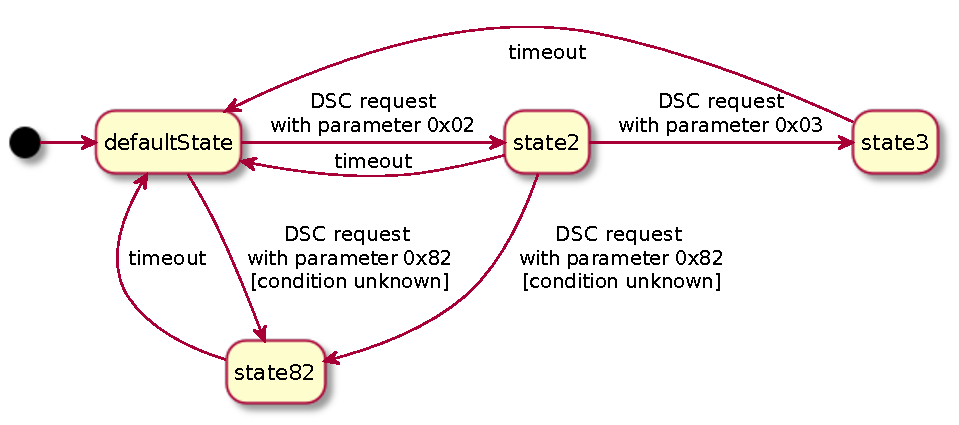
\includegraphics[width=0.7\textwidth]{uml/dsc-state-machine}
    \caption{Partial result for a PenTester of a UDS scan.}
    \label{fig:state-machine-of-scan}
\end{figure}

\subsection{Staged enumerators combine enumerators into a staged execution}

So-called staged enumerators contain enumerators where each enumerator is a stage. They start executing the first enumerator for each state, followed by each subsequent enumerator in the same way (see \autoref{fig:uml-staged-enumerators}).


\begin{figure}[htb]
    \centering
    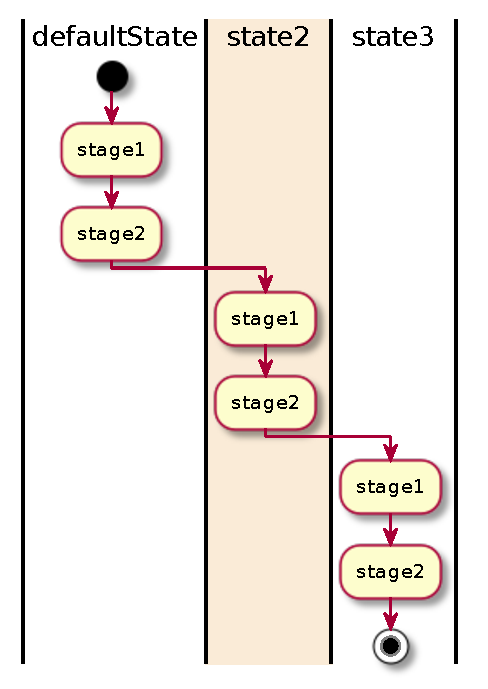
\includegraphics[width=0.35\textwidth]{uml/staged-enumerators}
    \caption{The sequence of a two-staged enumerator for three states.}
    \label{fig:uml-staged-enumerators}
\end{figure}

For each stage transition connectors can be defined. They are functions with two arguments, containing the previous enumerator and the new enumerator. Here, the results of the previous enumerator can be evaluated and the next enumerator can be configured accordingly. The connector will be automatically called by the UDS Scanner and expects a dictionary as return value that will be passed to the next enumerator. In \autoref{fig:uml-staged-enumerators}, the blue arrow represents the call of the connector. \autoref{lst:staged-enumerator} shows a simple definition of a staged enumerator.

\begin{listing}[H]
\begin{minted}
[frame=single,
framerule=0pt,
framesep=2mm,
baselinestretch=1.2,
bgcolor=VeryLightGray,
fontsize=\footnotesize,
linenos]
{python}
class MyStagedEnumerator(StagedAutomotiveTestCase):
    @staticmethod
    def connector_stage1_stage2(stage1_enum, stage2_enum):
        results = stage1_enum.get_results()
        stage2_config = create_config(results)
        return stage2_config
    
    def __init__(self):
        super().__init__(
            [Stage1Enumerator(), Stage2Enumerator()],
            # First element in the connectors list is never called because there is
            # no connection from nothing to stage 1. Only actual stages are connected.
            connectors=[None, self.connector_stage1_stage2])
\end{minted}
\caption{Example implementation of a two-staged enumerator.}
\label{lst:staged-enumerator}
\end{listing}

%\newpage

\subsection{Inheritance tree of the enumerators}

\begin{figure}[htb]
    \centering
    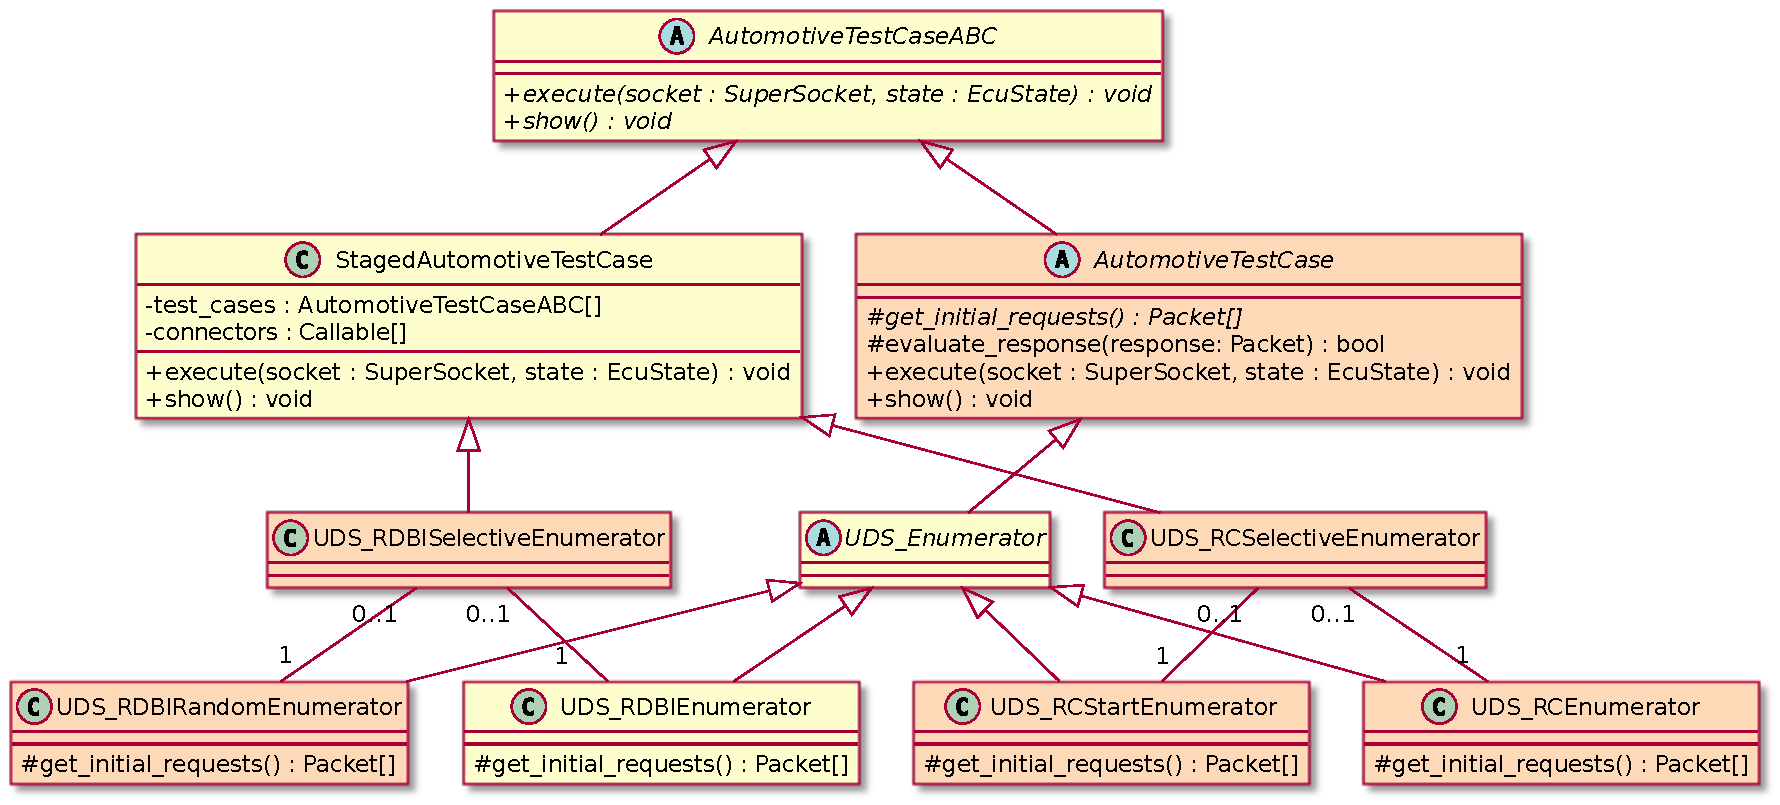
\includegraphics[width=1\textwidth]{uml/enumerators}
    \caption{Class diagram of enumerators.}
    \label{fig:uml-enumerators}
\end{figure}

\autoref{fig:uml-enumerators} shows the class tree of enumerators and their super classes. The classes with a darker background were modified or newly created for this thesis. Due to lack of space the configuration parameter of \mintinline{python}{get_initial_requests} was discarded. The full diagram can be seen in \autoref{app:uml}.

In general, scanners execute automotive test cases. For a regular UDS scan, these test cases are only service enumerators. However, other test cases are also conceivable, for example for fuzzing.

The root class of each enumerator is \mintinline{python}{AutomotiveTestCaseABC}. This is the type that is expected from scanners (see \autoref{fig:uml-scanners}). Staged enumerators inherit from \mintinline{python}{StagedAutomotiveTestCase} and single enumerators from \mintinline{python}{AutomotiveTestCase}. The \mintinline{python}{UDS_Enumerator} defines UDS-specific behavior that it doesn't need to be specified again for each UDS enumerator. For example, how the negative response code (NRC) of a negative response is read.

\mintinline{python}{AutomotiveTestCaseABC} requires each subclass to implement the \mintinline{python}{execute} method. Its first parameter \mintinline{python}{socket} specifies on which socket the requests and responses are communicated. \mintinline{python}{SuperSocket} is the root class of Scapy for all sockets. For the UDS Scanner, this is usually an \mintinline{python}{ISOTPSocket}.


\subsection{Scanner classes}

\begin{figure}[htb]
    \centering
    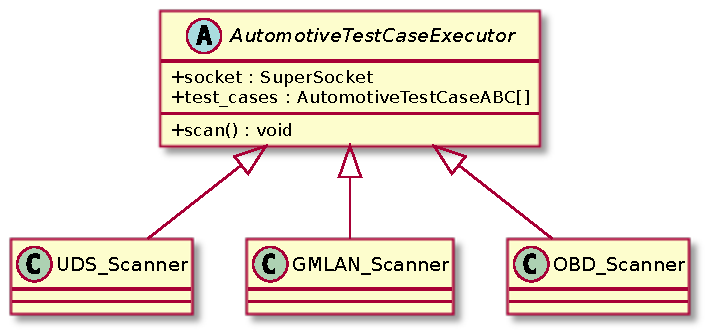
\includegraphics[width=0.6\textwidth]{uml/scanners}
    \caption{Class diagram of the protocol scanners.}
    \label{fig:uml-scanners}
\end{figure}

\autoref{fig:uml-scanners} shows the class diagram of the three protocol scanners in Scapy. Each is given a list of test cases (see \autoref{fig:uml-enumerators}) and a socket that is passed to each test case's \mintinline{python}{execute} method. Their \mintinline{python}{scan} method starts the scan.

\newpage

\section{Implementing enumerators for the RC service}

Three classes are of interest:

\begin{itemize}
    \item \mintinline{python}{RCEnumerator}: Defaults to scanning the whole RC service, including all three types.
    \item \mintinline{python}{RCStartEnumerator}: Only scanning type1 of the RC service.
    \item \mintinline{python}{RCSelectiveEnumerator}: Staged enumerator containing an RCStartEnumerator and an RCEnumerator.
\end{itemize}

For this work, the configurability of the \mintinline{python}{RCEnumerator} was improved, and the \mintinline{python}{RCStartEnumerator} and \mintinline{python}{RCSelectiveEnumerator} were created. \autoref{fig:rc-schematic} provides an initial overview of the new implementation mechanisms.

\begin{figure}[htb]
    \centering
    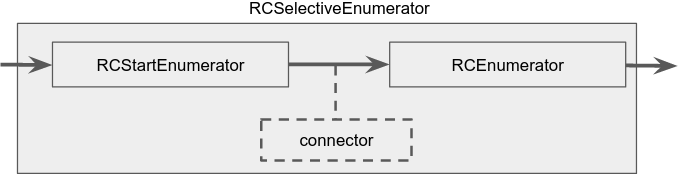
\includegraphics[width=0.7\textwidth]{rc-schematic}
    \caption{Schematic illustration of the new \mintinline{python}{RCSelectiveEnumerator}.}
    \label{fig:rc-schematic}
\end{figure}

First, the \mintinline{python}{RCEnumerator} will be explained by having a closer look at its \mintinline{python}{get_initial_requests} method.

\begin{listing}[H]
\begin{minted}
[frame=single,
framerule=0pt,
framesep=2mm,
baselinestretch=1.2,
bgcolor=VeryLightGray,
fontsize=\footnotesize,
linenos]
{python}
class UDS_RCEnumerator(UDS_Enumerator):
    def _get_initial_requests(self, **kwargs):
        type_list = kwargs.pop("type_list", [1, 2, 3])
        scan_range = kwargs.pop("scan_range", range(0x10000))

        return (
            UDS() / UDS_RC(routineControlType=rc_type,
                           routineIdentifier=data_id)
            for rc_type, data_id in itertools.product(type_list, scan_range)
        )
\end{minted}
\caption{The extended enumerator for the RC service.}
\label{lst:rc-enumerator}
\end{listing}

Two parameters can be configured, the \mintinline{python}{type_list} and \mintinline{python}{scan_range}. Both default to the values required to scan the whole RC service. Eventually, the method returns a generator that generates all requests possible by pairing the values of \mintinline{python}{type_list} and \mintinline{python}{scan_range}. This accomplishes the \mintinline{python}{itertools.product} method from the Python Standard library. It returns the cartesian product of the input iterables.

Next, the \mintinline{python}{RCStartEnumerator}.

\begin{listing}[H]
\begin{minted}
[frame=single,
framerule=0pt,
framesep=2mm,
baselinestretch=1.2,
bgcolor=VeryLightGray,
fontsize=\footnotesize,
linenos]
{python}
class UDS_RCStartEnumerator(UDS_RCEnumerator):
    def _get_initial_requests(self, **kwargs):
        kwargs["type_list"] = [1]
        return super()._get_initial_requests(**kwargs)
\end{minted}
\caption{The enumerator for the RC service scanning only type1.}
\label{lst:rc-start-enumerator}
\end{listing}

Its \mintinline{python}{get_initial_requests} method is simple. It fixes the \mintinline{python}{type_list} to type1 and then calls its implementation of the super class, which is the previously explained \mintinline{python}{UDS_RCEnumerator}. This results in generating requests only for type1.

The \mintinline{python}{UDS_RCSelectiveEnumerator} connects both of these enumerators.

\begin{listing}[H]
\begin{minted}
[frame=single,
framerule=0pt,
framesep=2mm,
baselinestretch=1.2,
bgcolor=VeryLightGray,
fontsize=\footnotesize,
linenos]
{python}
class UDS_RCSelectiveEnumerator(StagedAutomotiveTestCase):
    expansion_width = 253

    @staticmethod
    def connector_start_to_full(rc_start, rc_full):
        identifiers_with_pr = [r.resp.routineIdentifier for r
                            in rc_start.results_with_positive_response]

        scan_range = points_to_ranges(
            identifiers_with_pr, UDS_RCSelectiveEnumerator.expansion_width)

        return {"type_list": [2, 3],
                "scan_range": scan_range}

    def __init__(self):
        super().__init__(
            [UDS_RCStartEnumerator(), UDS_RCEnumerator()],
            [None, self.connector_start_to_full])
\end{minted}
\caption{The staged enumerator combining the start and complete enumerator for the RC service.}
\label{lst:rc-selective-enumerator}
\end{listing}

This staged enumerator has the \mintinline{python}{RCStartEnumerator} as the first stage, and the \mintinline{python}{RCEnumerator} as the second and last stage.
The expansion width is fixed to \textbf{253} as it was elaborated in \autoref{subsubsec:rc-elaborating}.

The connector calls \mintinline{python}{points_to_ranges} to expand the found identifiers of the first stage to ranges and passes them to the second stage. In addition, the connector configures the \mintinline{python}{RCEnumerator} to scan only type2 and type3, since type1 should no longer be scanned.

\begin{listing}[H]
\begin{minted}
[frame=single,
framerule=0pt,
framesep=2mm,
baselinestretch=1.2,
bgcolor=VeryLightGray,
fontsize=\footnotesize,
linenos]
{python}
def points_to_ranges(points, expansion_width):
    generators = []
    for identifier in points:
        start = max(identifier - expansion_width, 0)
        end = min(identifier + expansion_width + 1, 0x10000)
        generators.append(range(start, end))
    ranges_with_overlaps = itertools.chain.from_iterable(generators)
    return sorted(set(ranges_with_overlaps))
\end{minted}
\caption{Function extending points to ranges.}
\label{lst:points-to-ranges}
\end{listing}

\mintinline{python}{points_to_ranges} expands points to ranges and also resolves any overlaps to a continuous range.
First, a range generator is created for each given point. Then, they are chained and converted to a set, removing potential overlaps. This set is sorted in a list, to ensure understandable candump logs of a scan.

\section{Implementing enumerators for the RDBI service}

Again, three classes are of interest:

\begin{itemize}
    \item \mintinline{python}{RDBIEnumerator}: Defaults to scanning the whole RDBI service.
    \item \mintinline{python}{RDBIRandomEnumerator}: Scanning block-based with random identifiers.
    \item \mintinline{python}{RDBISelectiveEnumerator}: Staged enumerator containing an RDBIRandomEnumerator and an RDBIEnumerator.
\end{itemize}

The new implementation is two-staged. First, the \mintinline{python}{RDBIRandomEnumerator} is executed. Then, the connector creates requests for whole blocks, if any of their requests were answered positively, and ensured that for a single block each identifier is queried only once. The resulting requests are passed to the configurable \mintinline{python}{RDBIEnumerator}. \autoref{fig:rdbi-schematic} shows that schematically.

\begin{figure}[htb]
    \centering
    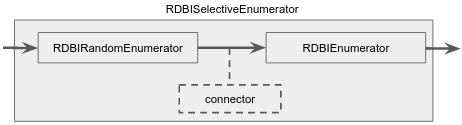
\includegraphics[width=0.7\textwidth]{rdbi-schematic}
    \caption{Schematic illustration of the new \mintinline{python}{RDBISelectiveEnumerator}.}
    \label{fig:rdbi-schematic}
\end{figure}

The explanation starts with the original enumerator, here the \mintinline{python}{RDBIEnumerator}.

\begin{listing}[H]
\begin{minted}
[frame=single,
framerule=0pt,
framesep=2mm,
baselinestretch=1.2,
bgcolor=VeryLightGray,
fontsize=\footnotesize,
linenos]
{python}
class UDS_RDBIEnumerator(UDS_Enumerator):
    def _get_initial_requests(self, **kwargs):
        scan_range = kwargs.pop("scan_range", range(0x10000))
        return (UDS() / UDS_RDBI(identifiers=[x]) for x in scan_range)
\end{minted}
\caption{The enumerator scanning the whole RDBI service by default.}
\label{lst:rdbi-enumerator}
\end{listing}

Since the RDBI service has only one parameter, its \mintinline{python}{get_initial_requests} remains simple, generating RDBI requests for identifiers from 0 to 65,535, if not configured otherwise.

Implementing the \mintinline{python}{RDBIRandomEnumerator} was a challenge because it must include the count of requests for each block. With a block size of \textbf{64} (see \autoref{subsubsec:rdbi-behavior}), there would need to be a list with $\frac{2^{16}}{64} = 1024$ elements. Thus, it is desirable to represent this information more compactly. A better representation is based on the fact that at least one request should be generated for each block. So, the number of samples is not stored for all blocks, but only for blocks whose number of samples is greater than or equal to two. And for blocks for which no value is stored, the value one is derived. This automatically solves that each block is probed with at least one request. These simplifications transformed the list of 1024 elements into a dictionary of only 109 elements. The non-simplified version is shown in \autoref{app:random-not-compact}.

\begin{listing}[H]
\begin{minted}
[frame=single,
framerule=0pt,
framesep=2mm,
baselinestretch=1.2,
bgcolor=VeryLightGray,
fontsize=\footnotesize,
linenos]
{python}
class UDS_RDBIRandomEnumerator(UDS_RDBIEnumerator):
    def _get_initial_requests(self, **kwargs):
        samples_per_block = {
            4: 29, 5: 22, 6: 19, 8: 11, 9: 11, 10: 13, 11: 14,
            # [...]
            1013: 14, 1014: 15
        }
        to_scan = []
        block_size = UDS_RDBIRandomEnumerator.block_size
        for block_index, start in enumerate(range(0, 2 ** 16, block_size)):
            end = start + block_size
            count_samples = samples_per_block.get(block_index, 1)
            to_scan += random.sample(range(start, end), count_samples)

        positive_identifiers = [t.resp.dataIdentifier for t in
                                self.results_with_positive_response]
        to_scan += positive_identifiers

        to_scan = sorted(list(set(to_scan)))
        return (UDS() / UDS_RDBI(identifiers=[x]) for x in to_scan)
\end{minted}
\caption{The enumerator scanning randomly the RDBI service based on blocks.}
\label{lst:rdbi-random-enumerator}
\end{listing}

The \mintinline{python}{random.sample} function from the Python Standard library returns a list of given length with unique elements chosen from the given sequence.

The implementation exploits the observation that most identifiers are available in multiple states. Thus, the randomly generated identifiers are appended with the identifiers that were answered positively in any previous state.

Again, the \mintinline{python}{UDS_RDBISelectiveEnumerator} brings these two enumerators together.

\begin{listing}[H]
\begin{minted}
[frame=single,
framerule=0pt,
framesep=2mm,
baselinestretch=1.2,
bgcolor=VeryLightGray,
fontsize=\footnotesize,
linenos]
{python}
class UDS_RDBISelectiveEnumerator(StagedAutomotiveTestCase):
    block_size = 2 ** 6

    @staticmethod
    def connector_random_to_sequential(rdbi_random, rdbi_full):
        identifiers_with_pr = \
            [r.resp.dataIdentifier
            for r in rdbi_random.results_with_positive_response]

        scan_range = points_to_blocks(
                identifiers_with_pr,
                UDS_RDBISelectiveEnumerator.block_size)
        return {"scan_range": scan_range}

    def __init__(self):
        super().__init__(
            [UDS_RDBIRandomEnumerator(), UDS_RDBIEnumerator()],
            [None, self.connector_random_to_sequential])
\end{minted}
\caption{The staged enumerator combining the random and complete enumerator for the RDBI service.}
\label{lst:rdbi-selective-enumerator}
\end{listing}

Since it is similar to the \mintinline{python}{RCSelectiveEnumerator}, it will not be explained any further. Only the \mintinline{python}{points_to_blocks} will be described in more detail.

\begin{listing}[H]
\begin{minted}
[frame=single,
framerule=0pt,
framesep=2mm,
baselinestretch=1.2,
bgcolor=VeryLightGray,
fontsize=\footnotesize,
linenos]
{python}
def points_to_blocks(points, block_size):
    generators = []
    for start in range(0, 2 ** 16, block_size):
        end = start + block_size
        pr_in_block = any((start <= identifier < end
                           for identifier in points))
        if pr_in_block:
            # Add generator creating all identifiers of a block
            generators.append(range(start, end))
    # Merge the generators
    scan_range = itertools.chain.from_iterable(generators)
    return scan_range
\end{minted}
\caption{Function extending points to fixed blocks.}
\label{lst:points-to-blocks}
\end{listing}

Unlike \mintinline{python}{points_to_ranges}, its block boundaries are fixed. It traverses each block and checks if any of the given identifiers is part of that block. If this is the case, the block will be scanned completely.

Unfortunately, this can lead to double-scanned identifiers, since instead of scanning only the remaining identifiers that have not yet been scanned in the respective blocks, the entire blocks are rescanned. Although an attempt was made to implement this, the UDS Scanner does not provide the necessary interfaces to do so. Executing the connectors also for state transitions or grouping generated UDS requests by ECU states would be required to create UDS requests per state. However, the connectors are only executed for stage transitions (see \autoref{fig:uml-staged-enumerators}), and the \mintinline{python}{get_initial_requests} method does not take a state argument. So, neither of these functions are provided by the UDS Scanner. Nevertheless, the number of duplicate requests is small, so the request savings hardly decrease.

\newpage

\section{Extending the enumerators to skip unsupported services}

In contrast to the previous approaches, this one is not applied to specific service enumerators, but to their super class \mintinline{python}{AutomotiveTestCase}. It evaluates each response, for example to detect if a new state was found. Here, a check was added for negative responses if they have a negative response code (NRC) of \mintinline{text}{0x11} or \mintinline{text}{0x7f}. If they do, the enumerator is set to completed for the currently executed state.

\begin{listing}[H]
\begin{minted}
[frame=single,
framerule=0pt,
framesep=2mm,
frame=single,
framerule=0pt,
framesep=2mm,
baselinestretch=1.2,
bgcolor=VeryLightGray,
fontsize=\footnotesize,
linenos]
{python}
class AutomotiveTestCase(AutomotiveTestCaseABC):
    """Base class for Enumerators"""

    def _evaluate_response(self, response, **kwargs):

        # Removed code for simplification

        # Negative responses contain the SID 0x7f
        # Must not be confused with the NRC
        if exit_if_service_not_supported and response.service == 0x7f:
            response_code = self._get_negative_response_code(response)
            if response_code in [0x11, 0x7f]:
                # Execution for current state is completed,
                # because a serviceNotSupported NR was received
                current_state = self._results[-1].state
                self._state_completed[current_state] = True
                # stop current execute and exit
                return True

        # Removed code for simplification

        return False
\end{minted}
\caption{The extended super class of each enumerator with skipping unsupported services.}
\label{lst:enumerator-super-class}
\end{listing}    
